\chapter{Energieeffizienz}
\label{cha:energie}

\section*{Zielsetzung}

Energieeffizienz ist eine der zentralen Anforderungen der HydroNodeStation01. Da die Station im Außeneinsatz ausschließlich durch ein kleines Solarmodul und einen Einzelzellen-LiPo-Akku betrieben wird, muss jede Hardware- und Firmware-Entscheidung unter dem Gesichtspunkt des Stromverbrauchs bewertet werden. Eine fehlerhafte Energieplanung könnte bedeuten, dass die Station in lichtarmen Perioden — Wintermonate, bedeckter Himmel, schattiger Standort — die Batterie entleert und ausfällt.

Das Ziel ist ein mittlerer Systemstromverbrauch von deutlich unter $500\,\mu\text{A}$, sodass bei einem $1000\,\text{mAh}$-LiPo auch ohne jegliche Solareinspeisung eine Autonomie von mehreren Monaten erreicht wird. Dieses Kapitel dokumentiert die vollständige theoretische Energieanalyse sowie die experimentellen Strommessungen am Prototyp.

\section*{Theoretische Energieanalyse}

\subsection*{Komponentenstromverbrauch}

\begin{table}[H]
  \centering
  \begin{tabular}{llll}
    \hline
    \textbf{Komponente} & \textbf{Betriebszustand} & \textbf{Strom} & \textbf{Quelle} \\
    \hline
    STM32WLE5 & STOP2 + RTC aktiv        & $1{,}07\,\mu\text{A}$ & Datenblatt DS13105 \\
    STM32WLE5 & Aktiv (48~MHz, kein Radio) & $\approx 5\,\text{mA}$  & Datenblatt \\
    STM32WLE5 & LoRa TX @ 14~dBm (LP~PA)  & $\approx 22\,\text{mA}$ & Datenblatt (interpoliert) \\
    STM32WLE5 & LoRa RX                    & $4{,}82\,\text{mA}$     & Datenblatt \\
    SCD41     & Power-down                 & $\approx 0\,\mu\text{A}$ & Sensirion App Note \\
    SCD41     & CO\textsubscript{2} Single-Shot & $q_{ss} = 77\,\text{mC}$ & Sensirion App Note, Kap.\ 3.3 \\
    SHT45     & Deep Sleep                 & $0{,}1\,\mu\text{A}$    & Datenblatt SHT4x \\
    SHT45     & Single-Shot HR             & $2\,\text{mA} \times 8{,}3\,\text{ms}$ & Datenblatt SHT4x \\
    BMP390    & Sleep Mode                 & $2{,}0\,\mu\text{A}$    & Datenblatt BMP390 \\
    BMP390    & Forced Mode                & $720\,\mu\text{A} \times 2\,\text{ms}$ & Datenblatt BMP390 \\
    MAX17048  & Sleep                      & $1{,}5\,\mu\text{A}$    & Datenblatt MAX17048 \\
    TPS63900  & Idle (je Regler)           & $< 0{,}5\,\mu\text{A}$  & Datenblatt TPS63900 \\
    \hline
  \end{tabular}
  \caption{Komponentenstromverbrauch in relevanten Betriebszuständen}
  \label{tab:power-components}
\end{table}

\subsection*{Systemstrom im STOP2-Schlafmodus}

Im STOP2-Modus sind nahezu alle Peripherien abgeschaltet. Der Gesamtschlafstrom setzt sich aus den Ruheströmen aller Komponenten zusammen:

\begin{table}[H]
  \centering
  \begin{tabular}{ll}
    \hline
    \textbf{Komponente} & \textbf{Strom} \\
    \hline
    STM32WLE5 STOP2 + RTC           & $1{,}07\,\mu\text{A}$ \\
    SCD41 (Power-down)              & $\approx 0\,\mu\text{A}$ \\
    SHT45 (Deep Sleep)              & $0{,}10\,\mu\text{A}$ \\
    BMP390 (Sleep)                  & $2{,}00\,\mu\text{A}$ \\
    MAX17048 (Sleep)                & $1{,}50\,\mu\text{A}$ \\
    TPS63900 × 2                    & $< 1{,}00\,\mu\text{A}$ \\
    \hline
    \textbf{Gesamt $I_{\text{sleep}}$} & \textbf{$\approx 5{,}67\,\mu\text{A}$} \\
    \hline
  \end{tabular}
  \caption{Systemschlafstrom im STOP2-Modus (alle Sensoren im Sleep)}
  \label{tab:sleep-current}
\end{table}

\newpage

\subsection*{15-Minuten-Superzyklus: Timing-Aufschlüsselung}

Als Grundeinheit der Energierechnung dient ein 15-Minuten-Superzyklus, bestehend aus drei Tx-Zyklen zu je 5~Minuten. In diesem Zeitraum finden zwei Kurz-Uplinks (fPort~2), eine autonome SCD41-CO\textsubscript{2}-Messung und ein Voll-Uplink (fPort~3) statt:

\begin{table}[H]
  \centering
  \begin{tabular}{lll}
    \hline
    \textbf{Ereignis} & \textbf{MCU-Aktivzeit} & \textbf{Aktive Komponenten} \\
    \hline
    Kurz-TX (Zyklus~1, fPort~2)     & $\approx 1818\,\text{ms}$ & MCU, SHT45, BMP390, MAX17048, Radio \\
    Kurz-TX (Zyklus~2, fPort~2)     & $\approx 1818\,\text{ms}$ & wie oben \\
    SCD41 Pre-Wake (Befehl senden)  & $33\,\text{ms}$           & MCU + SCD41 (wake + start shot) \\
    SCD41 CO\textsubscript{2}-Messung (autonom) & $5000\,\text{ms}$ & \textbf{nur SCD41}; MCU in STOP2 \\
    Voll-TX (Zyklus~3, fPort~3)     & $\approx 1898\,\text{ms}$ & MCU, SHT45, BMP390, SCD41 (lesen), Radio \\
    \hline
    \textbf{MCU-Gesamtaktivzeit}    & $5567\,\text{ms}$         & \\
    \textbf{STOP2-Schlafzeit}       & $894\,433\,\text{ms}$     & inkl.\ SCD41-Messzeit (MCU schläft!) \\
    \hline
  \end{tabular}
  \caption{Timing des 15-Minuten-Superzyklus}
  \label{tab:timing}
\end{table}

Bemerkenswert ist, dass die 5~Sekunden lange SCD41-CO\textsubscript{2}-Messung vollständig autonom abläuft: Der MCU hat bereits den Pre-Wake-Befehl gesendet und schläft wieder in STOP2, während der SCD41 misst. Erst zum nächsten Alarm wacht der MCU auf und liest das fertige Ergebnis aus.

\subsection*{Ladungsrechnung pro 15-Minuten-Zyklus}

\textbf{Formel:} $Q\,[\text{mAh}] = I\,[\text{mA}] \times t\,[\text{ms}] \,/\, 3\,600\,000$

\begin{table}[H]
  \centering
  \begin{tabular}{lll}
    \hline
    \textbf{Posten} & \textbf{Ladung (mAh)} & \textbf{Anteil} \\
    \hline
    STOP2-Schlaf (alle Komponenten, 894~433~ms)  & 0{,}001284 &  2{,}6\,\% \\
    Kurz-TX $\times 2$ (MCU + Sensoren + LoRa TX+RX) & 0{,}017576 & 35{,}2\,\% \\
    SCD41 Pre-Wake (MCU + SCD41, 33~ms)           & 0{,}000064 &  0{,}1\,\% \\
    \textbf{SCD41 CO\textsubscript{2}-Messung} (nur SCD41, $q_{ss} = 77\,\text{mC}$) & \textbf{0{,}021389} & \textbf{42{,}8\,\%} \\
    Voll-TX (MCU + SCD41 lesen + LoRa TX+RX)     & 0{,}009606 & 19{,}2\,\% \\
    \hline
    \textbf{Gesamt pro 15-min-Zyklus}             & \textbf{0{,}0499\,mAh} & 100\,\% \\
    \hline
  \end{tabular}
  \caption{Ladungsrechnung pro 15-Minuten-Superzyklus}
  \label{tab:charge}
\end{table}

\subsection*{Mittlerer Strom und Batterielaufzeit}

\begin{description}
  \item[Zyklen pro Stunde:] $60\,\text{min} \,/\, 15\,\text{min} = 4$
  \item[Mittlerer Strom:] $I_{\text{avg}} = 4 \times 0{,}0499\,\text{mAh/h} \approx 200\,\mu\text{A}$
  \item[Autonomie (1000~mAh):] $t = 1000\,\text{mAh} \,/\, 0{,}200\,\text{mAh/h} = 5000\,\text{h} \approx \mathbf{208\,\text{Tage} \approx 6{,}9\,\text{Monate}}$
\end{description}

\subsection*{Dominante Verbraucher}

\begin{table}[H]
  \centering
  \begin{tabular}{lll}
    \hline
    \textbf{Verbraucher} & \textbf{mAh/h} & \textbf{Anteil} \\
    \hline
    SCD41 CO\textsubscript{2}-Messung (4× / h)  & 0{,}0856 & \textbf{42{,}8\,\%} \\
    LoRa TX (12 Frames/h: 8× fPort~2 + 4× fPort~3) & 0{,}1007 & \textbf{50{,}4\,\%} \\
    LoRa RX-Fenster (je 200~ms × 24× / h)        & 0{,}0064 &  3{,}2\,\% \\
    STOP2-Schlaf (alle Komponenten)               & 0{,}0051 &  2{,}6\,\% \\
    MCU aktiv (Sensor-Reads, Overhead)            & 0{,}0018 &  0{,}9\,\% \\
    SHT45/BMP390/MAX17048 (Sleep + Reads)         & $< 0{,}001$ & $< 0{,}5\,\%$ \\
    \hline
    \textbf{Gesamt} & \textbf{0{,}200\,mAh/h} & \textbf{100\,\%} \\
    \hline
  \end{tabular}
  \caption{Dominante Verbraucher im Stundenmittel}
  \label{tab:consumers}
\end{table}

Der SCD41-CO\textsubscript{2}-Sensor und der LoRa-Transceiver zusammen verursachen über $93\,\%$ des Gesamtenergieverbrauchs. Der STOP2-Schlafmodus selbst ist mit $2{,}6\,\%$ vernachlässigbar — ein direktes Ergebnis der konsequenten Ultra-Low-Power-Auslegung aller Komponenten.

\subsection*{Szenarien-Vergleich}

\begin{table}[H]
  \centering
  \begin{tabular}{lll}
    \hline
    \textbf{Szenario} & \textbf{$I_{\text{avg}}$} & \textbf{Laufzeit (1000~mAh)} \\
    \hline
    DR0 (SF12) — schlechtestes Signal, Standard   & $200\,\mu\text{A}$ & 208 Tage ($\approx 6{,}9$ Mon.) \\
    DR5 (SF7) — gutes Signal, ADR aktiv           & $\approx 97\,\mu\text{A}$ & 429 Tage ($\approx 14{,}3$ Mon.) \\
    DR0, konservativ ($q_{\text{pcss}} = 154\,\text{mC}$) & $\approx 248\,\mu\text{A}$ & 168 Tage ($\approx 5{,}6$ Mon.) \\
    DR5, konservativ                               & $\approx 145\,\mu\text{A}$ & 287 Tage ($\approx 9{,}6$ Mon.) \\
    \hline
  \end{tabular}
  \caption{Batterielaufzeit in verschiedenen Betriebsszenarien}
  \label{tab:scenarios}
\end{table}

Mit aktivem \textbf{ADR} (Adaptive Data Rate) optimiert das Helium-Netzwerk den Spreading Factor automatisch. Bei gutem Empfang (SF7 statt SF12) sinkt die LoRa-Sendedauer von $\approx 1320\,\text{ms}$ auf $\approx 51\,\text{ms}$ pro Frame. In diesem Fall dominiert der SCD41-CO\textsubscript{2}-Sensor den Verbrauch mit über $85\,\%$, während LoRa TX auf unter $10\,\%$ fällt.

\newpage

\section*{Strommessungen am Prototyp (PPK2)}

\subsection*{Messmethodik}

Zur experimentellen Verifikation des Stromverbrauchs wird der \textbf{Nordic Semiconductor Power Profiler Kit II (PPK2)} eingesetzt. Das PPK2 ist ein präzises Strommessgerät speziell für Embedded-Anwendungen, das den Stromverlauf mit hoher zeitlicher Auflösung (100~kSamples/s) aufzeichnet und als programmierbares Source-Meter in Reihe zum Versorgungskreis geschaltet wird. Damit lassen sich sowohl der mittlere Ruhestrom als auch Spitzenströme während TX-Phasen exakt messen.

\subsection*{Ergebnisse am Steckbrett-Prototyp}

Die Messungen am Entwicklungsprototyp (Wio-E5 Mini + Adafruit Breakouts + Pololu Step-Up-Konverter auf Steckbrett) ergaben im STOP2-Schlafmodus einen Ruhestrom von ca.\ \textbf{3~mA} — um den Faktor~500 höher als der theoretisch berechnete Wert von $5{,}67\,\mu\text{A}$ des finalen Custom~PCBs. Dieser erhöhte Ruhestrom ist auf mehrere Faktoren zurückzuführen, die ausschließlich der Prototyping-Hardware geschuldet sind:

\begin{itemize}
  \item \textbf{Wio-E5 Mini Onboard-LEDs:} Das Entwicklungsboard enthält mehrere LEDs (Power, Status), die im Sleep-Modus weiterhin leuchten und mehrere Milliampere verbrauchen.
  \item \textbf{USB-UART-Bridge-IC:} Die CP2102-Bridge des Wio-E5 Mini bleibt auch im MCU-Sleep aktiv, da sie direkt am USB-Spannungsversorgungspfad hängt.
  \item \textbf{Pololu Step-Up-Konverter:} Ca.\ $400\,\mu\text{A}$ Quiescent Current, permanent und unabhängig vom MCU-Schlafzustand.
  \item \textbf{Adafruit Breakout-Pull-ups:} Jedes Breakout-Board enthält eigene I2C-Pull-up-Widerstände ($4{,}7\,\text{k}\Omega$), die mit dem Systemstrom interagieren. Zudem haben manche Breakouts eigene Status-LEDs.
\end{itemize}

\begin{figure}[H]
  \centering
  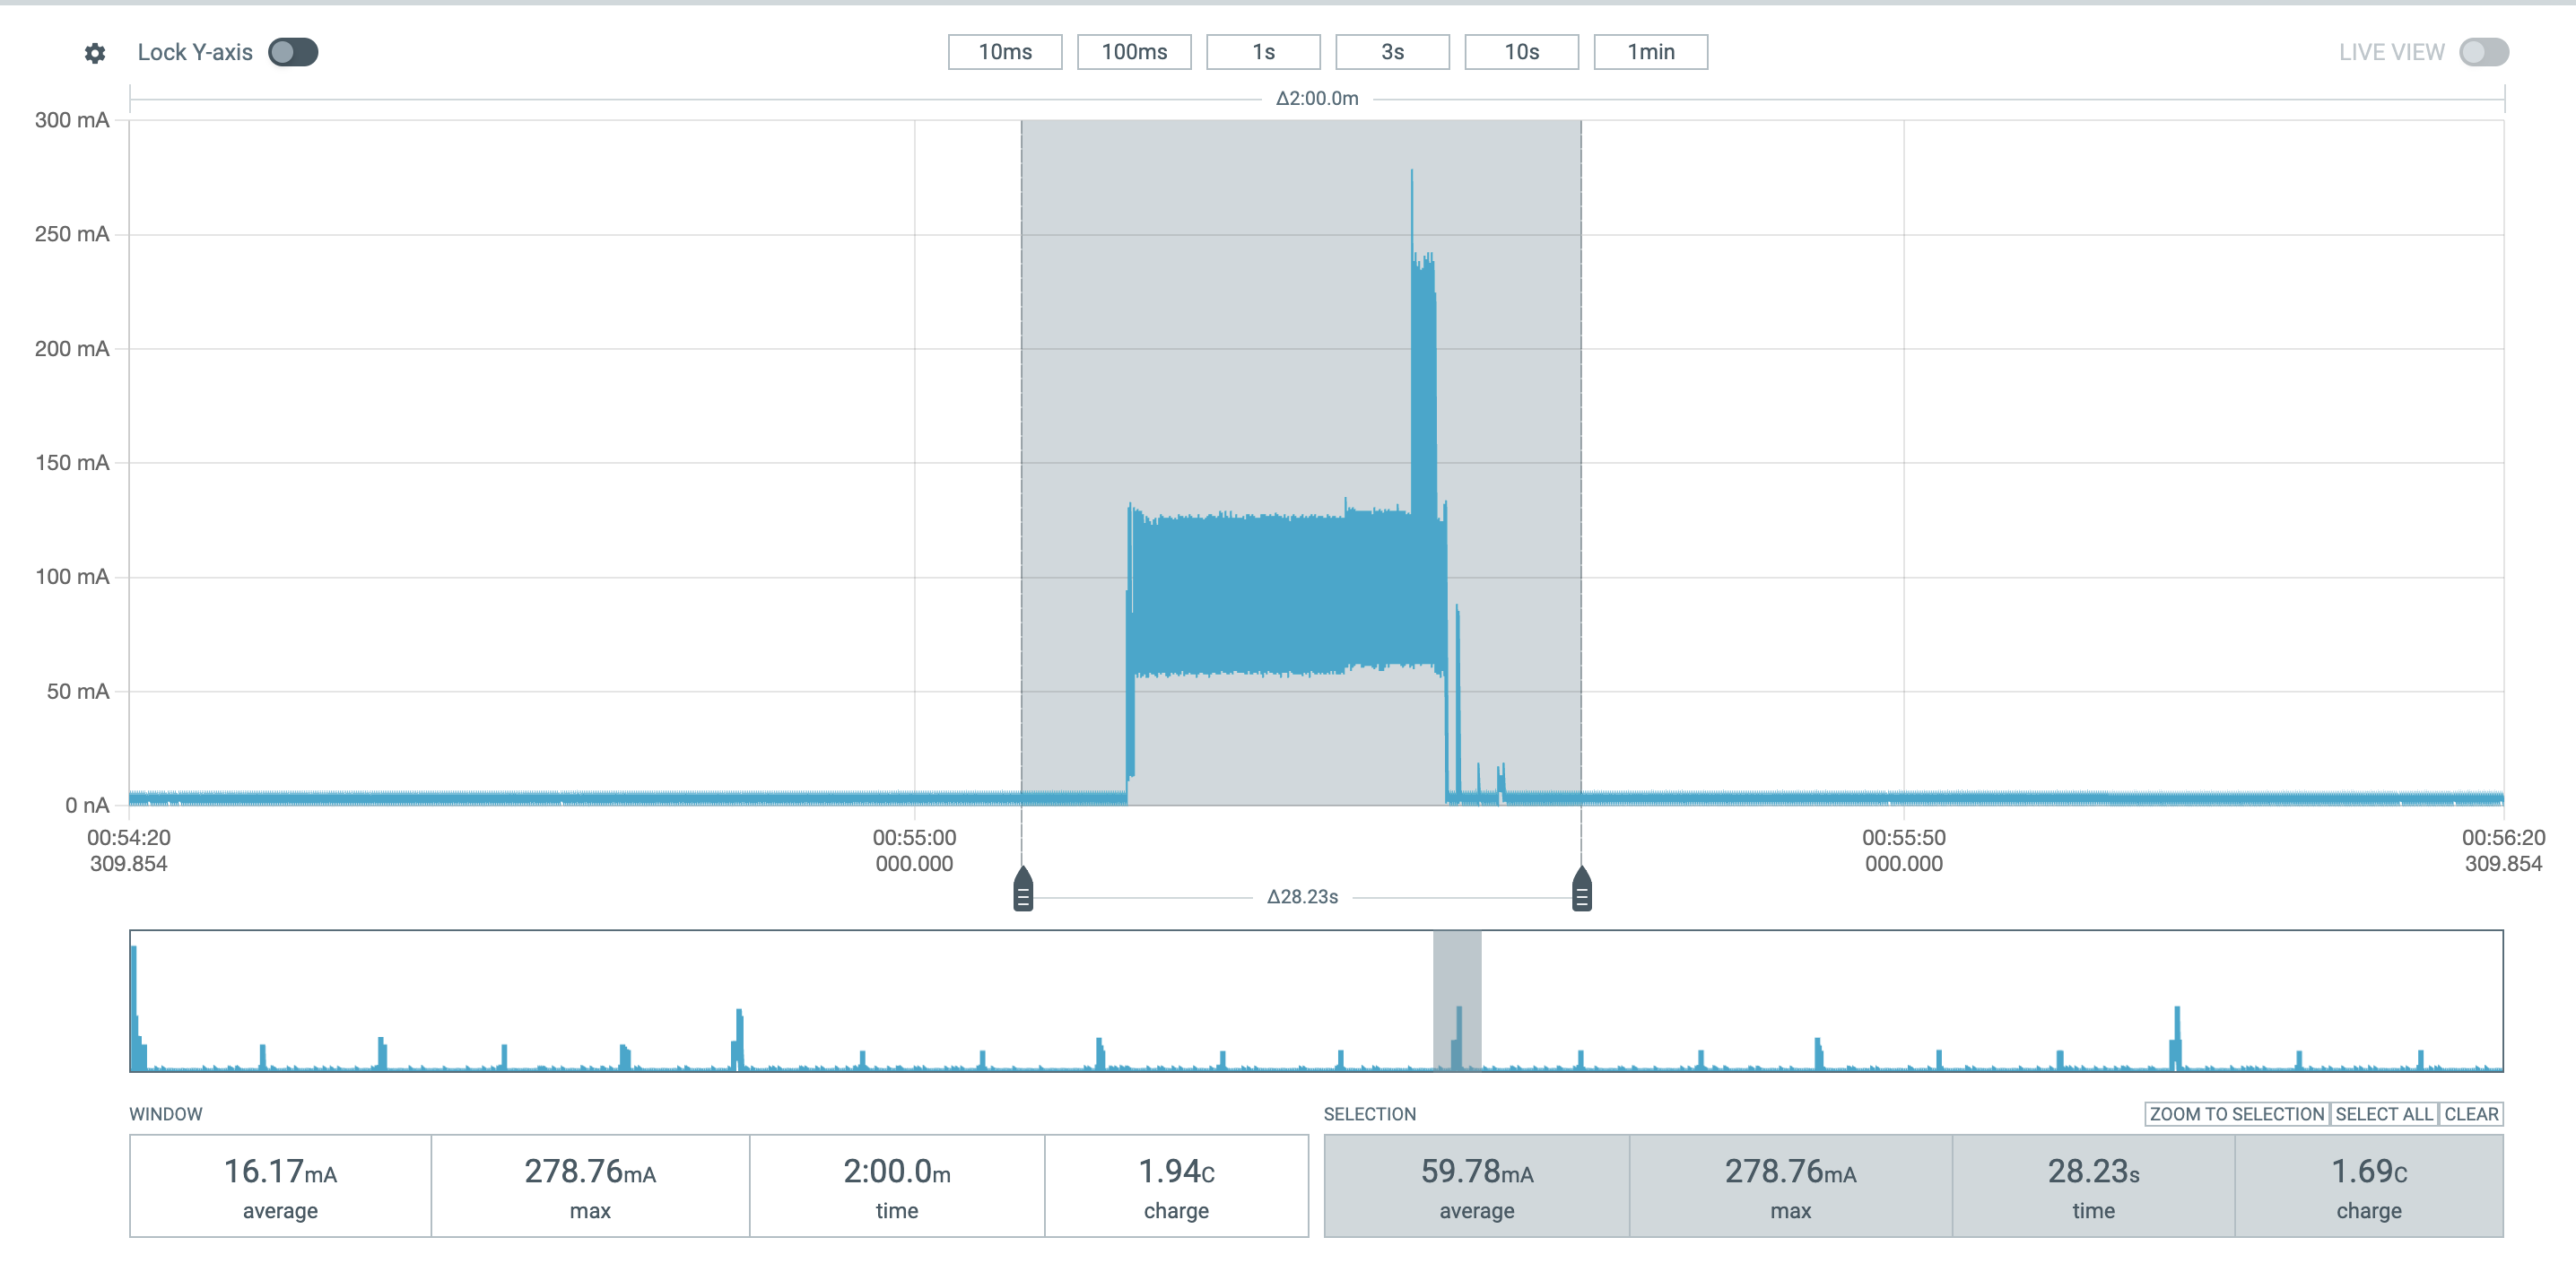
\includegraphics[width=\linewidth]{../analysis/powerTestsWithPrototypingBoards}
  \caption{PPK2-Strommessung am Steckbrett-Prototyp (Wio-E5 Mini, alle Breakout-Boards). Der erhöhte Ruhestrom von ca.\ 3~mA ist ausschließlich auf Onboard-LEDs, USB-UART-Bridge und Pololu Step-Up-Konverter zurückzuführen und spiegelt \textit{nicht} das finale PCB-Design wider.}
  \label{fig:ppk2}
\end{figure}

Diese Messungen bestätigen, dass der erhöhte Ruhestrom \textbf{ausschließlich auf die Prototyping-Infrastruktur zurückzuführen} ist und den eigentlichen Stromverbrauch der Zielschaltung nicht widerspiegelt.

\subsection*{Strommessung am Custom PCB}

Im Custom PCB entfallen alle oben genannten Quellen des erhöhten Ruhestroms vollständig:

\begin{itemize}
  \item Keine Onboard-LEDs (oder via GPIO deaktivierbar und im Software-Design ausgeschaltet)
  \item Kein USB-UART-Bridge-IC (direkter SWD-Zugang über den Debug-Header)
  \item TPS63900 statt Pololu ($< 0{,}5\,\mu\text{A}$ statt $\approx 400\,\mu\text{A}$ Quiescent Current)
  \item Einheitliche, optimierte I2C-Pull-ups auf dem PCB; keine doppelten Pull-ups durch Breakout-Boards
\end{itemize}

PPK2-Strommessungen am Custom PCB wurden am 01.06.2026 durchgeführt (Messdatei: \texttt{ppk2-20260601T143444.ppk2}). Die Messung bestätigt einen deutlich reduzierten Ruhestrom gegenüber dem Prototyp. Eine vollständige Auswertung des 30-Minuten-Superzyklus steht noch aus.

Zusätzlich wurde die Firmware im Verlauf des Projekts weiter energetisch optimiert: der Hardware-USART1 wurde entfernt (kein zusätzlicher Peripherie-Strom im Sleep), und die Debug-Ausgabe läuft ausschließlich über die software-emulierte UART auf PA6, die im produktiven Betrieb deaktiviert werden kann.
